%%%%%%%%%%%%%%%%%%%%%%%%%%%%%%%%%%%%%%%%%%%%%%%%%%%%%%%%%%%%%%%%%%%%%%%%%%%
%%                      Couverture report LaTeX template                 %%
%%%%%%%%%%%%%%%%%%%%%%%%%%%%%%%%%%%%%%%%%%%%%%%%%%%%%%%%%%%%%%%%%%%%%%%%%%%

\documentclass[a4paper,12pt,twoside]{article}
\usepackage{couverture}
\usepackage[T1]{fontenc}
%% \usepackage[french]{babel}
\usepackage[latin1]{inputenc}
\usepackage{url}
\usepackage{amssymb}
\usepackage{amsmath}
\usepackage{subfigure}

\usepackage{tikz}
\usetikzlibrary{arrows,positioning}

\newcommand{\couv}{{\sc Couverture}}
\renewcommand{\le}{\leqslant}
\renewcommand{\ge}{\geqslant}
\newcommand{\N}{\mathbb{N}}
\newcommand{\anysc}{\star}
\newcommand{\andthen}{\texttt{and then}}
\newcommand{\orelse}{\texttt{or else}}
\newcommand{\adanot}{\texttt{not}}

%%%%%%%%%%%%%%%%%%%%%%%%%%%%%%%%%%%%%%%%%%%%%%%%%%%%%%%%%%%%%%%%%%%%%%%%%%%%%%

\newtheorem{theorem}{\textsc{Theorem}}
\newtheorem{lemma}{Lemma}[subsection]

\def\@begintheorem#1#2{\trivlist
   \item[\hskip \labelsep{#1\ #2}]\itshape}

\begin{document}
\pagestyle{empty}

\vfill

\begin{center}%
{\Large \textbf{\couv{}}}

{\Large \textbf{Technical Report on OBC/MCDC properties}}

\vfill

{\large \textbf{Abstract}}
\end{center}

This document gathers results established or formalized by the \couv{}
project team about relationships between specific coverage criteria.
%
We focus in particular on how \E{Object Branch Coverage} (OBC) relates to the
\E{Modified Condition/Decision Coverage} (MCDC) criterion.

We provide two broad categories of results: formal proofs of important
properties over a model of the two criteria, and a machine-automated
verification of some of these properties for concrete subsets of the model
expressed in Alloy.
%
These results constitute the grounds on which our project coverage analysis
framework operates to infer source coverage results from object coverage
information out of an instrumented execution environment.

\vfill

\newpage
\pagestyle{plain}

%%%%%%%%%%%%%%%%%%%%%%%%%%%%%%%%%%%%%%%%%%%%%%%%%%%%%%%%%%%%%%%%%%%%%%%%%%%%%%

\section{Common definitions}

\subsection{Decisions, conditions}

We are considering decisions that are short circuit boolean expressions,
i.e. expressions consisting in elementary boolean conditions combined
together using only the \andthen{}, \orelse{} and \adanot{} operators.

For each decision we construct the associated ROBDD (Reduced Ordered
Binary Decision Diagram), whose nodes are conditions. (RO)BDDs have an
entry point, and two or more exit edges labeled True and False.

\subsection{Binary decision diagrams}

In the remainder of this document, unless otherwise indicated, all
references to BDDs denote reduced ordered BDDs.

\subsection{Coverage metrics}

\subsubsection{Definitions}

% define MC/DC, OBC, BDDBC

This document deals with properties of tests exercising object code under
the assumption that the code generation chain accurately preserves the
decision process captured in the ROBDD. We specifically assume when
discussing object branch coverage of the object code, that we can instead
reason, unless indicated explicitly, on (RO)BDD branch coverage
of the corresponding BDD.

\subsection{Minimal test sets}

Coverage assessment is accomplished by exercising some piece of object
code in a variety of test cases, recording data along the way, and
then determining whether the successive executions of the object code
satisfy a given criterion of exhaustiveness. The minimum number of distinct
executions required to achieve a specific criterion is an important
aspect in the evaluation of any coverage assessment methodology. Here
we establish some properties that give a hard limit on test set size
for various coverage metries.

\subsubsection{OBC}

\subsubsection{MC/DC}

\begin{theorem}
MC/DC on a decision with $n$ independent conditions is achieved with
a test set of exactly $n+1$ tests, and cannot be achieved in fewer tests.
\end{theorem}

The existence of the test set is proved by induction. For one condition,
MC/DC is achieved with two tests, one setting it True and the other False.

Now assume that the property holds for all $n \le{} N$, and consider a decision
with $N+1$ conditions. It is of the form $D = D_l \anysc{} D_r$ where
$\anysc{}$ is either \andthen{} or \orelse{}. There is also possibly a
negation, which is omitted here since it has no impact on MC/DC. For the
remainder of this proof we assume the operator is \andthen{}; the same
reasoning applies similarly for the case of \orelse{}.

$D_l$ and $D_r$ are decisions with respectively $n_l$ and $n_r$ conditions
(both at most $N$), and $n_l + n_r = N+1$. From the induction hypothesis
we have two test vector sets $T_l = \{ v_l (0) .. v_l (n_l) \}$ and
$T_r = \{ v_r (0) .. v_r (n_r) \}$ that satisfy MC/DC for $D_l$ and $D_r$
respectively, and we can arbitrarily choose the indices so that
$D_l$ is True for $v_l(0)$ and $D_r$ is True for $v_r (0)$.

We can now create a combined test set for the complete decision as follows.
$$(\forall j \in [0, n_l])\, v (j) = (v_l (j) \cdot v_r (0))$$
$$(\forall j \in [1, n_r])\, v (n_l + j) = (v_l (0) \cdot v_r (j))$$

We have thus created a set $T = \{ v(0) .. v(n_l + n_r) \}$ of $N+2$ tests.
It is immediate that the elements with indices 0 to $n_l$ give for D
the same outcome as the corresponding elements of $T_l$ for $D_l$,
and they all have identical values for the conditions coming from $D_r$,
so they show independent influence of all conditions coming from $D_l$.
Similarly the vector set $\{v(0), v(n_l+1) .. v(n_l + n_r)\}$ shows
independent influence of those conditions coming from $D_r$, so the new
test set $T$ satisfies MC/DC for $D$ and thus the induction property holds at
$N+1$ as well, since $T$ has $n_l + n_r + 1 = N+2$ elements.

The proof that this is the minimal test set size is given in~\cite{ar0118}.

\subsection{Coverage assessment through analysis of execution traces}


\section{Characterization of cases of BDDBC --- MC/DC equivalence}

This section discusses the distinction between expressions for which
BDDBC of the associated ROBDD implies MC/DC, and expressions for which
no such implication holds.

\subsection{Some cases of non equivalence between OBC and MC/DC}

First let us have a look at how MC/DC and object coverage relate to each
other on some simple cases. Cases of non-equivalence for decisions with up to
5 conditions have been studied in \cite{ar0720}: non-equivalence cases
have been shown to occur in decisions with three or more conditions,
and an illustration is provided with (A \andthen{} B) \orelse{} C,
where A, B and C are three independent conditions.
%
A representation of this decision's BDD is depicted on
figure~\ref{subfig:D1}:

\begin{figure}[h]
\centering

\begin{tabular}{cc}

\subfigure[]{
  \label{subfig:D1}
  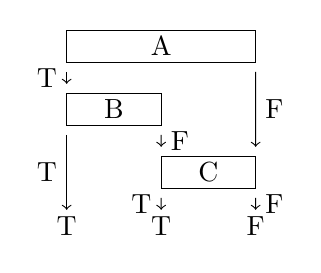
\begin{tikzpicture}[scale=0.8]

    \draw (0,0) rectangle node {A} (3,-0.5);
    \node at (0,-0.5) (if_a_true) {};
    \node at (3,-0.5) (if_a_false) {};

    \draw (0,-1) rectangle node {B} (1.5,-1.5);
    \node at (0,-1)   (b_left) {};
    \node at (1.5,-1)   (b_right) {};
    \node at (0,-1.5) (if_b_true) {};
    \node at (1.5,-1.5) (if_b_false) {};

    \draw (1.5,-2) rectangle node {C} (3,-2.5);
    \node at (1.5,-2)   (c_left) {};
    \node at (3,-2)   (c_right) {};
    \node at (1.5,-2.5) (if_c_true) {};
    \node at (3,-2.5) (if_c_false) {};

    \node at (0, -3) (outcome_true1) {};
    \node at (1.5, -3) (outcome_true2) {};
    \node at (3, -3) (outcome_false) {};

    \node at (0, -3.1) (outcome_true1_label) {T};
    \node at (1.5, -3.1) (outcome_true2_label) {T};
    \node at (3, -3.1) (outcome_false_label) {F};

    \draw [->] (if_a_true)  -- node[left] {T} (b_left);
    \draw [->] (if_a_false) -- node[right] {F} (c_right);

    \draw [->] (if_b_true)  -- node[left] {T} (outcome_true1);
    \draw [->] (if_b_false) -- node[right] {F} (c_left);

    \draw [->] (if_c_true)  -- node[left] {T} (outcome_true2);
    \draw [->] (if_c_false) -- node[right] {F} (outcome_false);

  \end{tikzpicture}
} & \subfigure[]{
  \label{subfig:D2}
  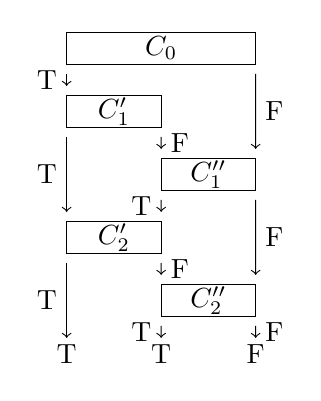
\begin{tikzpicture}[scale=0.8]

    \draw (0,0) rectangle node {$C_{0}$} (3,-0.5);
    \node at (0,-0.5) (if_c0_true) {};
    \node at (3,-0.5) (if_c0_false) {};

    \draw (0,-1) rectangle node {$C'_{1}$} (1.5,-1.5);
    \node at (0,-1)   (c1a_left) {};
    \node at (1.5,-1)   (c1a_right) {};
    \node at (0,-1.5) (if_c1a_true) {};
    \node at (1.5,-1.5) (if_c1a_false) {};

    \draw (1.5,-2) rectangle node {$C''_{1}$} (3,-2.5);
    \node at (1.5,-2)   (c1b_left) {};
    \node at (3,-2)   (c1b_right) {};
    \node at (1.5,-2.5) (if_c1b_true) {};
    \node at (3,-2.5) (if_c1b_false) {};

    \draw (0,-3) rectangle node {$C'_{2}$} (1.5,-3.5);
    \node at (0,-3)   (c2a_left) {};
    \node at (1.5,-3)   (c2a_right) {};
    \node at (0,-3.5) (if_c2a_true) {};
    \node at (1.5,-3.5) (if_c2a_false) {};

    \draw (1.5,-4) rectangle node {$C''_{2}$} (3,-4.5);
    \node at (1.5,-4)   (c2b_left) {};
    \node at (3,-4)   (c2b_right) {};
    \node at (1.5,-4.5) (if_c2b_true) {};
    \node at (3,-4.5) (if_c2b_false) {};

    \node at (0, -5) (outcome_true1) {};
    \node at (1.5, -5) (outcome_true2) {};
    \node at (3, -5) (outcome_false) {};

    \node at (0, -5.1) (outcome_true1_label) {T};
    \node at (1.5, -5.1) (outcome_true2_label) {T};
    \node at (3, -5.1) (outcome_false_label) {F};

    \draw [->] (if_c0_true)  -- node[left] {T} (c1a_left);
    \draw [->] (if_c0_false) -- node[right] {F} (c1b_right);

    \draw [->] (if_c1a_true)  -- node[left] {T} (c2a_left);
    \draw [->] (if_c1a_false) -- node[right] {F} (c1b_left);

    \draw [->] (if_c1b_true)  -- node[left] {T} (c2a_right);
    \draw [->] (if_c1b_false) -- node[right] {F} (c2b_right);

    \draw [->] (if_c2a_true)  -- node[left] {T} (outcome_true1);
    \draw [->] (if_c2a_false) -- node[right] {F} (c2b_left);

    \draw [->] (if_c2b_true)  -- node[left] {T} (outcome_true2);
    \draw [->] (if_c2b_false) -- node[right] {F} (outcome_false);

  \end{tikzpicture}
}\\
\end{tabular}

\caption{Example decision BDDs}
\label{fig:examples}
\end{figure}

From this representation, we can see that a set of three evaluations can
achieve branch coverage of the whole BDD, corresponding to the three vertical
paths in figure~\ref{subfig:D1}.
%
These evaluations are:

\begin{center}
\begin{tabular}{|c|c|c||c|}
\hline
A & B & C & (A \andthen{} B) \orelse{} C \\ \hline
T & T & x & T \\ \hline
T & F & T & T \\ \hline
F & x & F & F \\ \hline
\end{tabular}
\end{center}

where ``x'' means not evaluated and thus can be indifferently True or False.
%
Now, indeed, even though all the BDD edges are covered, MC/DC is not met. In
particular, the independent effect of conditions B and C on the decision is
not shown.  Since $n+1$ tests are needed to cover a decision with $n$
condition with respect to MC/DC, 3 evaluations cannot cover a three-condition
decision.

It turns out that this particular case can be generalized in a
quite spectacular counterexample: there exists classes of decisions
with an arbitrary high number of conditions that can be branch covered
by just three evaluations; the previous example was one element of this
class with 3 conditions.

Consider the following set $\{D_{n}\}_{n \in \N}$  of decisions:

\begin{itemize}
\item let $D_{0}$ be a simple condition decision; by convention,
      we will call $C_{0}$ its condition;
\item let us define $D_{n}$, for any $n>0$, as follows:\\
      $D_{n} = (D_{n-1} \ \andthen{} \ C'_{n}) \ \orelse{} \ C''_{n}$\\
      $C'_{n}$ and $C''_{n}$ being independent from each other and from
      any condition in $D_{n-1}$.
\end{itemize}

In other words:
\begin{itemize}
\item $D_{0} = C_{0}$
\item $D_{1} = (C_{0} \ \andthen{} \ C'_{1}) \ \orelse{} \ C''_{1}$
\item $D_{2} = (((C_{0} \ \andthen{} \ C'_{1}) \ \orelse{} \ C''_{1})\\
                 \andthen{} \ C'_{2}) \ \orelse{} \ C''_{2}$
\item $D_{3} = (((((C_{0} \ \andthen{} \ C'_{1}) \ \orelse{} \ C''_{1})\\
                 \andthen{} \ C'_{2}) \ \orelse{} \ C''_{2})\\
                   \andthen{} \ C'_{3}) \ \orelse{} \ C''_{3}$
\item ...
\end{itemize}

Figure~\ref{subfig:D2} shows the BDD for $D_{2}$, where it is visible
that all the edges can be covered by three evaluation paths which only
demonstrate the independent effect of $C_{0}$:

\begin{center}
\begin{tabular}{|c|c|c|c|c||c|}
\hline
$C_{0}$   & $C'_{1}$   & $C''_{1}$   & $C'_{2}$   & $C''_{2}$   & $D_{2}$ \\ \hline
T      & T       & x        & T       & x        & T     \\ \hline
T      & F       & T        & F       & T        & T     \\ \hline
F      & x       & F        & x       & F        & F     \\ \hline
\end{tabular}
\end{center}

We can thus build a decision $D_{n}$ with an arbitrary number of conditions,
that can be BDD branch covered by just three evaluation paths. As MC/DC can
only be achieved with a minimal number of $n+1$ evaluations, this is a
striking case where BDD branch coverage (and consequently OBC) is far from
being equivalent to MC/DC.

We can now adopt a more general perspective and characterize more
precisely the difference between these two criteria.

\subsection{Construction of the ROBDD}

The BDD we associate with a decision is constructed using the following
recursive procedure:

\begin{description}
\item[Build\_BDD.Condition]
  The BDD for a decision consisting in a single condition C has the node
  "test C" as its entry point, the label True is assigned to the branch
  corresponding to "C is True", and the label False is assigned to the
  branch corresponding to "C is False".

\item[Build\_BDD.NOT]
  The BDD for $\adanot{} (D)$ is the BDD for D where the labels of the exit
  edges have been swapped.

\item[Build\_BDD.Short\_Circuit\_Operator]
  This rule defines how the BDD for $(D1) \anysc{} (D2)$ is constructed for
  any short-circuit operator $\anysc{}$.

  If $\anysc{}$ is \andthen{}, let SC be False
  If $\anysc{}$ is \orelse{}, let SC be True

  Let B1 be the BDD for D1, and B2 the BDD for D2.

  Then B, the BDD for D is obtained by combining B1 and B2 as follows:
  \begin{itemize}
    \item the entry point is that of B1
    \item the exit edge labeled SC of B1 is an exit edge labeled SC of B
    \item the other exit edge of B1 connects to the entry point of B2
    \item the exit edges of B2 are exit edges of B with the same labels
  \end{itemize}
\end{description}

The following invariants of ROBDDs follow from the construction process:
\begin{itemize}
  \item There is exactly one BDD node for each condition.
  \item All condition nodes are reachable (i.e. there is a path from
        the entry point to any node in the BDD).
  \item There are no cycles in the BDD.
  \item Both outcomes are reachable (i.e. there is a path from the entry point
        to an exit edge labeled True and to an exit edge labeled False).
\end{itemize}

\subsection{Evaluation of a decision}

Given the transformation of a decision into its ROBDD, evaluating the
decision consists in computing its value using the following BDD traversal
procedure:

\begin{description}
\item[Eval.Condition]
  The value of a decision that consists in a lone condition is the
  value of the condition.

\item[Eval.Not]
  To evaluate $\adanot{} (D)$, evaluate D and take the opposite value

\item[Eval.Short\_Circuit\_Operator]
  To evaluate $(D1) \anysc{} (D2)$, evaluate D1. If $D1 = SC$ then the
  value is SC, else evaluate D2, and the value is that of D2.
\end{description}

The following property holds:

\begin{description}
\item[Evals\_Are\_Paths]
  Evaluating a decision is equivalent to traversing the BDD, evaluating
  each condition as BDD nodes are traversed, and using the label of the
  exit edge as the value of the decision.
\end{description}

This property, and most other properties that we'll discuss here,
is proved by recurrence on the number of binary operators involved in
the expression. We'll assume that it holds for all $n \le{} N$, and then
consider an expression with $N+1$ binary operators, and prove that
the BDD construction step Build\_BDD.Short\_Circuit\_Operator preserves
the property from the two subdecision BDDs to the overall BDD.

Note that the practical implementation of coverage analysis systems based
on control flow traces relies on the assumption that the code generator
used to produce executable code from expressions actually implements this
evaluation strategy.

\subsection{Outcome reachability}

XXX well-known property of ROBDDs, could be included in list
of invariants trivially following the construction process???

\subsection{Equivalence case}

We now consider the case of an expression whose BDD has no diamond path,
i.e. for each BDD node there is exactly one path from the entry point to
that node. The following property holds:

\begin{description}
\item[BDDBC\_No\_Diamond\_Indep\_Implies\_MCDC]
  For a BDD with no diamond, if conditions are independent, then
  BDD branch coverage implies masking MC/DC coverage.
\end{description}

Let's consider a condition C. Since we have BDD branch coverage,
all possible paths starting at C have been taken (by recurrence on path
length, taking advantage of no cycles and no diamonds).

From the independent outcome reachability property, we have two paths
starting at C, beginning each with one edge from C, and ending on the
two outcomes of the decision. Let's call them PCT and PCF.

These paths are disjoint: any condition appearing in one is masked
in the other (because of no-diamond).

These two paths are parts of paths PT and PF from the BDD entry point to
either outcome, and they cannot differ on the part of the path from the
entry point to C.

So, PT and PF differ in C, in no other condition before C, and in no
other non-masked condition after C, so they prove independent influence
of C over the decision.

This holds for each condition in the decision, so MC/DC is proved.

\subsection{Non-equivalence case}

Proved by constructing a set of paths that give BDD branch coverage but
not MC/DC coverage, taking advantage of the fact that we can reach the
same node C through two different paths.

% A candidate proof has been given here:
% http://lists.forge.open-do.org/pipermail/couverture-discuss/2010-May/000091.html

\subsection{Conclusion}

We have therefore proved the following property:

\begin{theorem}
  \label{thm:no-diamond}
  Given a decision D, branch coverage of the BDD implies MC/DC if,
  and only if, there is no diamond in the BDD (i.e.  no node of the
  BDD is reachable through more that one path from the root).
\end{theorem}

Intuitively, BDDBC is a local property of BDD traversals (i.e. of evaluations
of the decision): it is evaluated individually for each BDD node, without
respect to how the BDD node was reached. In contrast, MC/DC is a non-local
property, since it involves the complete path through the BDD. To establish
independent influence of condition C, it is necessary to study what happens
for two values of C leading to different outcomes, \emph{with all other
conditions fixed}, i.e. considering a single way of \emph{arriving to C}.

\section{A second characterization of the equivalence case}

In this section we provide an alternative (equivalent) property
that characterizes cases where BDD branch coverage implies MC/DC:

\begin{theorem}
  \label{thm:lhs-same-operator}
  Given a decision D, BDD branch coverage implies MC/DC if, and only if, when
  considering the negation normal form D' of D, for every sub-decision E of D',
  all binary operators in the left-hand-side operand of E, if any, are of the
  same kind as E's operator.
\end{theorem}

The negative normal form is obtained by rewriting the expression using
De Morgan's laws so that negations apply only to atomic conditions (and not
to more complex subexpressions).

We prove this theorem by showing that this alternative characterization is
equivalent to having no diamond in the associated BDD.
Theorem~\ref{thm:lhs-same-operator} follows by application of
Theorem~\ref{thm:no-diamond}.

Let's consider a decision D and its BDD. For the order of atoms in the
BDD, we take the order in which they appear in a depth-first traversal
of the decision (represented as a tree).

% ??? Add results about ordering...

\begin{figure}
\centering

\subfigure[$DL \ \orelse{} \ DR$]{
\label{subfig:DL-or-DR}
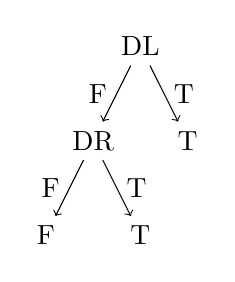
\begin{tikzpicture}[scale=0.8]
  \node (DL) {DL}
    child[->] {
      node (DR) {DR}
        child[->] {node (DRF) {F} edge from parent node[left] {F}}
        child[->] {node (DRT) {T} edge from parent node[right] {T}}
      edge from parent node[left] {F}
    }
    child[->] {node (DLT) {T} edge from parent node[right] {T}};
\end{tikzpicture}

%           DL
%        F / \ T
%         /   \
%        DR    T
%     F / \ T
%      /   \
%     F     T

}
\subfigure[$DL \ \andthen{} \ DR$]{
\label{subfig:DL-and-DR}
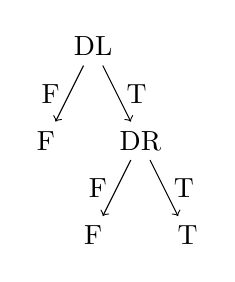
\begin{tikzpicture}[scale=0.8]
  \node (DL) {DL}
    child[->] {node (DLF) {F} edge from parent node[left] {F}}
    child[->] {
      node (DR) {DR}
        child[->] {node (DRF) {F} edge from parent node[left] {F}}
        child[->] {node (DRT) {T} edge from parent node[right] {T}}
      edge from parent node[right] {T}
    };
\end{tikzpicture}

%           DL
%        F / \ T
%         /   \
%        F     DR
%           F / \ T
%            /   \
%           F     T

}
\caption{case 2 and 3}
\end{figure}

There is a diamond in a BDD if and only if there is at least one node
such that the number of paths to reach it from root is strictly
greater than 1; we will use this caracterization to prove our
property.

\emph{Proof of the simplified case:}

Consider first the case where decision D does not contain any negation.
Each non-terminal node in the BDD corresponds to a sub-decision D' in D
(i.e. the root of each sub-decision is a non-terminal node in D's BDD).

\emph{Proof of reverse implication (simplified case):}

Let's call NF(D) the number of paths from the root of decision D to False (F)
and NT(D) the number of paths from the root of decision D to True (T).

\emph{case 1:} D = A (atom)\\
$NF(D) = NT(D) = 1$

\emph{case 2:} D = $DL \ \orelse{} \ DR$\\
The BDD for D can be constructed from the BDDs for DL and DR. It is shown 
in Figure~\ref{subfig:DL-or-DR}.


$NF(D) = NF(DL) * NF(DR)$\\
$NT(D) = NT(DL) + NF(DL) * NT(DR)$

\emph{case 3:} D = $DL \ \andthen{} \ DR$\\
The BDD for D can be constructed from the BDDs for DL and DR. It is shown 
in Figure~\ref{subfig:A-and-B}.

$NF(D) = NF(DL) + NT(DL) * NF(DR)$\\
$NT(D) = NT(DL) * NT(DR)$

\begin{lemma}
\label{lemma:NF-NT-bound}
For every E, $NF(D) \ge 1$ and $NT(D) \ge 1$.
If D is of the form \orelse{} then $NT(D) \ge 2$.
If D is of the form \andthen{} then $NF(D) \ge 2$.
\end{lemma}

\begin{lemma}
\label{lemma:NF-NT-monotonic}
NF and NT are monotonic functions, i.e. if D' is a sub-decision of D,
then we have
        $NF(D') \le NF(D)$
and        
        $NT(D') \le NT(D)$.
\end{lemma}

Proofs of Lemmas~\ref{lemma:NF-NT-bound} and~\ref{lemma:NF-NT-monotonic} are on
structural induction on the form of decisions, based on the three cases
distinguished above.

Then, suppose a decision D of the form \andthen{} contains a
sub-decision D' of the form \orelse{} on the left-hand side, of the form
\orelse{}. If DL, DR are the two sub-decisions such that
$D = DL \andthen{} DR$, then D' is also a sub-decision of DL.

By Lemma~\ref{lemma:NF-NT-bound}, we know that $NT(D') \ge 2$. By
Lemma~\ref{lemma:NF-NT-monotonic}, we know that $NT(DL) \ge NT(D')$.

Then, in D's BDD, the paths reaching the DR's root node are exactly
those paths in DL's BDD reaching True, by construction; the number of
these paths is NT(DL).

Thus, DR's root node in the D's BDD is reachable by more than one
path. As a consequence, there is a diamond in this BDD.

Similarly, if a decision D of the form \orelse{} contains a
sub-decision D' of the form \andthen{} on the left-hand side, we can
exhibit a non-terminal node in the BDD for D that is reachable by more
than one path.

By contraposition, if there are no diamonds in the BDD associated to a
decision D, then D has no \orelse{} sub-decision on the left of its
\andthen{} sub-decisions, and no \andthen{} sub-decision to the left of
its \orelse{} sub-decision.

\emph{Proof of implication (simplified case):}

Now suppose that for every sub-decision in decision D, the left
operand of an \andthen{} sub-decision contains only \andthen{}
sub-decisions and the left operand of an \orelse{} sub-decision
contains only \orelse{} sub-decisions.

\begin{lemma}
\label{lemma:NF-NT-only-one-oper}
If E contains only \orelse{} sub-decisions then $NF(E) = 1$.
If E contains only \andthen{} sub-decisions then $NT(E) = 1$.
\end{lemma}

Proof of Lemma~\ref{lemma:NF-NT-only-one-oper} is on structural induction on
the form of decisions, based on the 3 cases distinguished above.

By structural induction on the depth of the BDD, we can show that there cannot
be any diamond in the BDD associated to D, which proves that the desired
implication holds.

\emph{Proof of the general case:}

In the general case, decision D may contain \adanot sub-decisions. Then,
consider D' the negation normal form of D. Since D and D' are represented
by the same BDD, Theorem~\ref{thm:lhs-same-operator} follows.

\section{General stateless MC/DC assessment}

This section discusses a code transformation after which stateless BDDBC
traces carry sufficient information to assess MC/DC coverage.

\section{Automated verifications}

\newpage
\bibliographystyle{alpha}
\bibliography{couverture}

\end{document}
